This paper implements the workflow depicted in \fig{workflow} for modeling the RabbitMQ \cmt{broker} and conducting security analysis. 

\begin{figure}[h]
\noindent
     \centering
		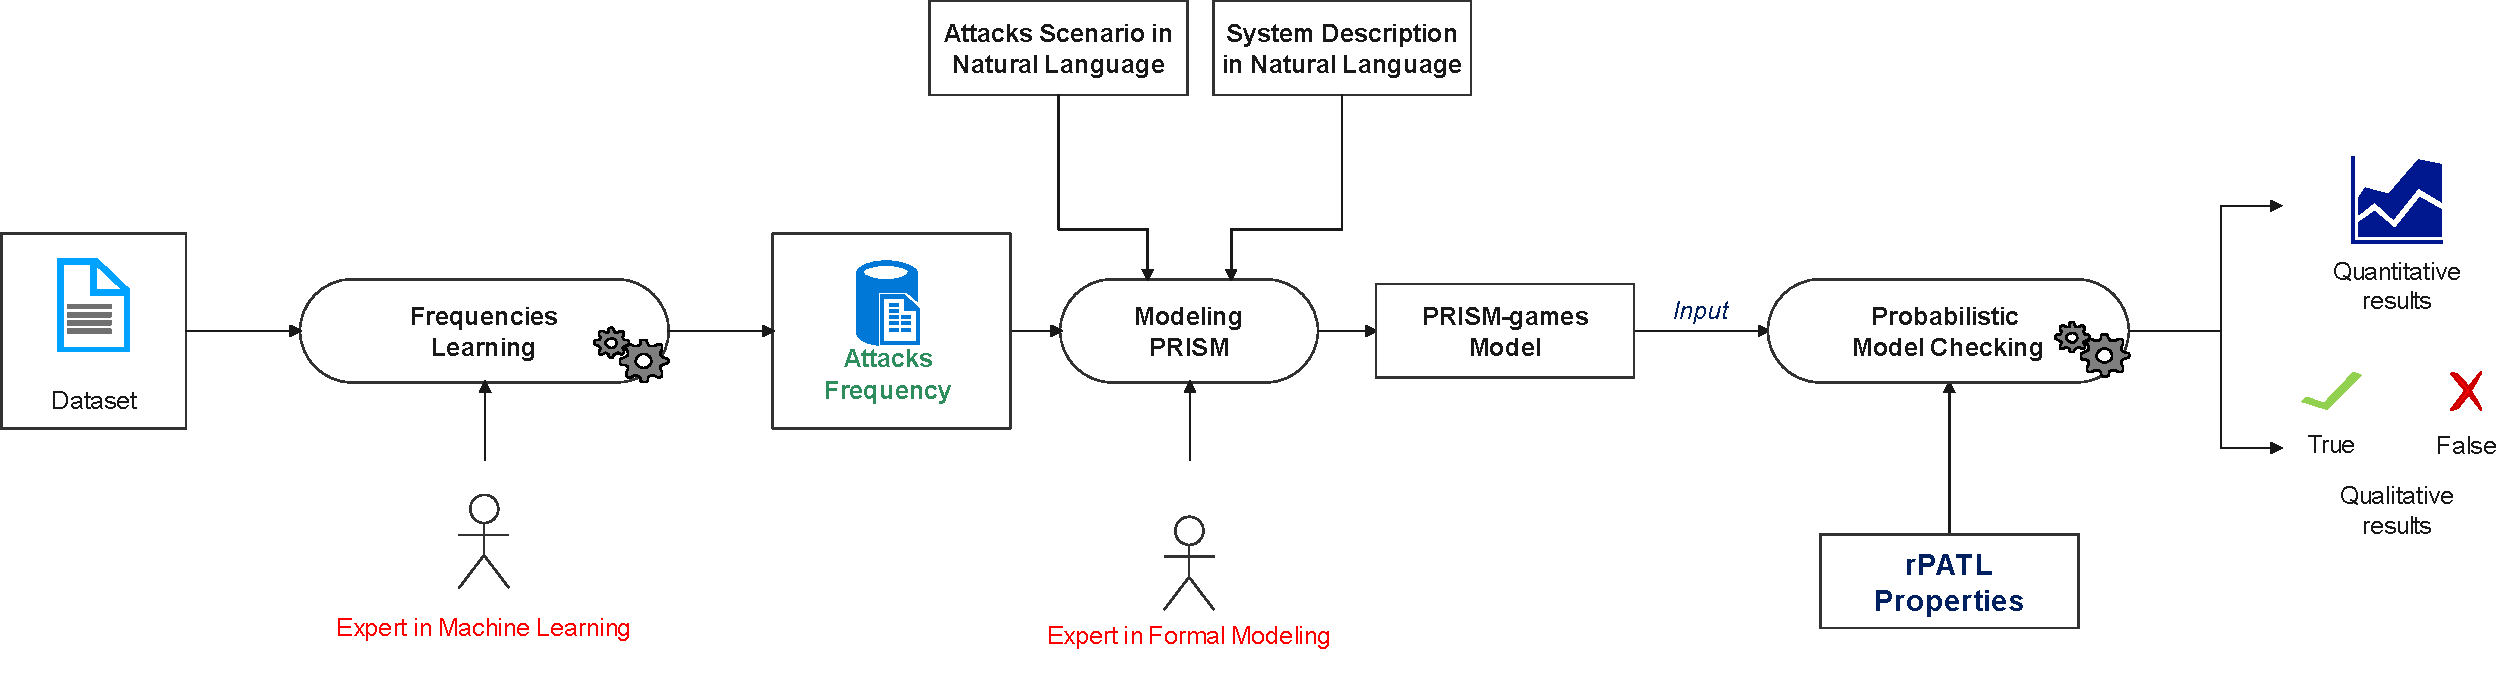
\includegraphics[width=470pt, height =150pt]{flow.pdf}
		\caption{A Workflow for Learning, Modeling, and Verification of the RabbitMQ \cmt{Broker}}
	\label{workflow}
\end{figure}



% Learning step : 
\paragraph{Frequencies learning} The frequencies of attacks, such as DoS, Mirai, and ARP spoofing, have been learned \cmt{from} a collected dataset using the algorithm described in Section \ref{frequencies}. These attack frequencies are required for populating the PRISM model.

\paragraph{Modeling} The modeling phase entails translating protocol specifications, described in natural language \cite{Rabbitmq}, into a PRISM model consisting of modules that adhere to the PRISM language (as discussed in Section \ref{Preliminaries}). This process results in a parametrizable PRISM model. Our work enhances this process by incorporating security considerations and formalizing specific attack scenarios within the CSG PRISM-supported language. The attack scenario examined in this research focuses on CAPEC-384 \cite{capec384}, which involves the \quot{\emph{Application API Message Manipulation via Man-in-the-Middle}}. Therefore, the parametrizable PRISM model is populated with attack frequencies to capture the stochastic nature of the attacks within their cyber-physical environment. These frequencies represent the occurrence of attacks as probabilistic phenomena derived from an Open-Source dataset. 

\paragraph{Probabilistic model checking} To assess the potential risks inherent in the RabbitMQ \cmt{broker} regarding attacks, we utilize rPATL properties. The risk involves assessing the likelihood of an attack occurring and its potential consequences on the communication protocol \cite{Grzegorz2011}. The rPATL properties provide an indication of the degree of data corruption in the \cmt{form} of game goals resulting from manipulated data within the \cmt{broker} using the PRISM-games model checker. By considering these properties, we gain insights into risks that may arise within the RabbitMQ \cmt{broker}. 





